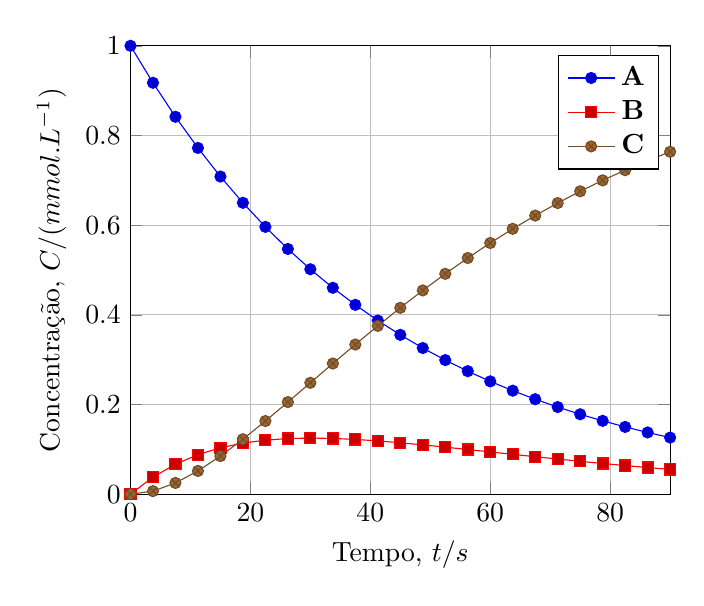
\begin{tikzpicture}
    \def\ka{0.023}
    \def\kb{0.046}
    \begin{axis}
        [
            grid = major,
            xlabel = {Tempo, $t/\si{s}$},
            ylabel = {Concentração, $C/(\si{mmol.L^{-1}})$},
            xmin = 0,  xmax=90, 
            ymin = 0, ymax = 1,
            domain = 0:90,
        ]
        \addplot
            {
              exp(-\ka*x)
            };
        \addplot
            {
              \ka/\kb*(exp(-\ka*x)-exp(-\kb*x))
            };
        \addplot
            {
              1+\ka/(\kb-\ka)*exp(-\kb*x)-\kb/(\kb-\ka)*exp(-\ka*x)
            };
        \legend{\textbf{A}, \textbf{B}, \textbf{C}}
    \end{axis}
\end{tikzpicture}